\newpage
\begin{center}
    \Huge{\textbf{\underline{Exercise 5}}}
\end{center}

\vspace{0.45cm}

\begin{center}
    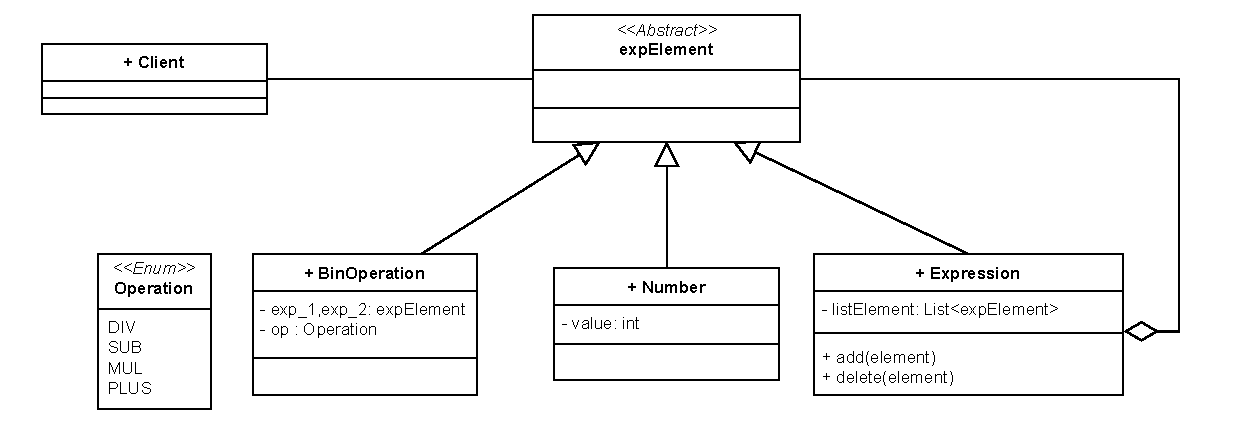
\includegraphics[height=0.22\textheight]{Exercices/EX5/ex5.drawio.pdf}
\end{center}

\vspace{0.25cm}


\begin{prettyBox}{Explication}{myblue}
The \texttt{Operation} is an \texttt{enum} class that represents the different arithmetic operations 
(\texttt{DIV}, \texttt{SUB}, \texttt{MUL}, \texttt{PLUS}).\\[0.15cm]
The \texttt{Number} class represents an integer value and serves as a leaf element.\\[0.15cm]
The \texttt{BinOperation} class is a composite element that holds two \texttt{expElement} instances 
(\texttt{exp\_1} and \texttt{exp\_2}), which can be either \texttt{Number}, another \texttt{BinOperation}. It also includes an \texttt{Operation} to define the arithmetic operator.\\[0.15cm]
Finally, the \texttt{Expression} class is a composite element that holds a list of \texttt{expElement} instances 
via the \texttt{listElement}. 
\end{prettyBox}

